\documentclass{sig-alternate-05-2015}

\usepackage{xcolor}
\usepackage{subcaption}
\captionsetup{font=bf}

\newcommand{\note}{\color{red}$*$}

\begin{document}

\tolerance=10000 

\title{A Synthesis-Aided Compiler for Manycore Computation}

\numberofauthors{1} 
\author{
\alignauthor
Alexa VanHattum\\
       \affaddr{Cornell University: CS 6410: Advanced Systems}\\
       \email{avh@cs.cornell.edu}
}
\date{1 November 2018}

\maketitle

\begin{abstract}

Novel, programmable computer architectures offer developers orders-of-magnitude performance improvements over traditional CPUs or GPUs for certain classes of computation, such as dense matrix computation. However, compiling programs to run on such hardware ``accelerators'' is an arduous task. An efficient, optimized compiler for a new architecture may take multiple engineer-years of work to build, much of which is specific only to that target accelerator. We are creating a compiler for a re-configurable, ``manycore'' architecture that partitions and maps computation across a grid of distinct, simple processor cores. Our compiler leverages program synthesis, a core programming languages technology used to automate the construction of programs, to spatially map computation without relying on traditional hand-written optimizations. We achieve a 3.3-5.0X speedup in estimated idealized cycle counts on microbenchmarks compared to a single-core execution. While our compiler does tread the limits of reasonable scalability for modern synthesis techniques, we are able to compile our largest microbenchmark (152 lines of code) to a non-optimal, but 1.7X faster, partitioning within  about an hour. This work aims to ultimately allow developers to write programs for new, efficient hardware accelerators without learning to write dense low-level code themselves or waiting for an optimized compiler to be developed via traditional mechanisms. In addition, we expect such synthesis-aided compiler technology to be more flexible for compiling to distinct but related architectures in the future.

\end{abstract}


%
% The code below should be generated by the tool at
% http://dl.acm.org/ccs.cfm
% Please copy and paste the code instead of the example below. 
%
\begin{CCSXML}
<ccs2012>
<concept>
<concept_id>10011007.10011006.10011041.10011043</concept_id>
<concept_desc>Software and its engineering~Retargetable compilers</concept_desc>
<concept_significance>500</concept_significance>
</concept>
<concept>
<concept_id>10011007.10011006.10011008.10011024.10011034</concept_id>
<concept_desc>Software and its engineering~Concurrent programming structures</concept_desc>
<concept_significance>500</concept_significance>
</concept>
</ccs2012>
\end{CCSXML}
\ccsdesc[500]{Software and its engineering~Retargetable compilers}
\ccsdesc[500]{Software and its engineering~Concurrent programming structures}

%
% End generated code
%

%
%  Use this command to print the description
%
\printccsdesc

\keywords{Program Synthesis, Compilers, Reconfigurable Architecture, Spatial Architecture}

\section{Introduction}
To create the most performant applications, software developers are increasingly exploring the use of programmable hardware accelerators. One promising style of accelerator (especially popular in embedded computing) combines many small, simple, independent processor cores. As one example of the excitement around this technology, Intel has described its 2016 Xeon Phi processor as a ``brand-new many-core architecture that delivers massive thread parallelism, data parallelism, and memory bandwidth in a CPU form factor for high-throughput workloads''~\cite{xeonphi}. While such ``manycore'' accelerators can offer huge performance gains, their use often necessitates unfamiliar and low-level programming models that may be hard for developers to navigate. For example, new hardware may be designed by computer architects to support only a language at about the same abstraction level as an assembly language but with additional unfamiliar syntax. Specialized compilers from high-level languages offer more programmability to application developers. However, because the design and manufacturing of specialized accelerators may be one-off, compiler engineers then find themselves in a race against time to optimize for an unfamiliar architecture that may be surpassed in a few short years. Further, it may take multiple engineer-years to develop an optimized compiler for a new architecture, leaving application developers without many options in the meantime beyond writing low-level code themselves.

% {\note Citation for first sentence?}

\begin{figure}
\centering
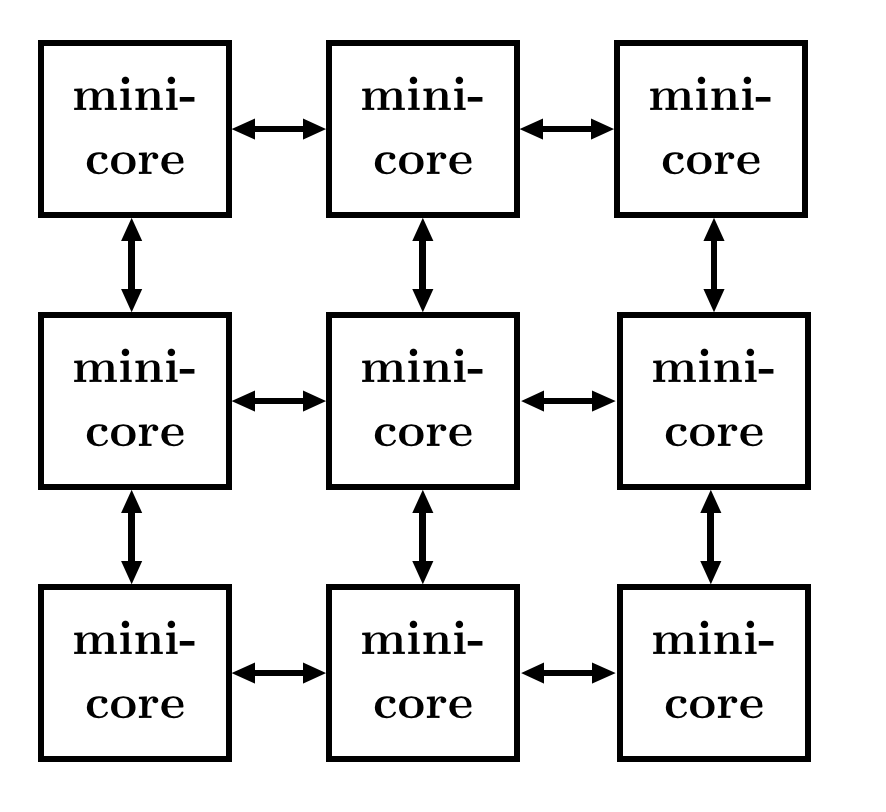
\includegraphics[width=1.7in]{core-grid.png}
\caption{A $3 \times 3$ grid of mini-cores processors. As shown, each core can only communicate directly with 4 (or fewer) immediately adjacent cores.}
\label{fig:core-grid}
\end{figure}

Compiling programs to run efficiently on a manycore architecture poses numerous challenges. First, unlike when compiling for a traditional CPU architecture, there is no underlying operating system that handles the scheduling of processes and threads across the several cores. Rather, it is the responsibility of either the programmer (if they are writing low-level code directly) or the compiler to partition and schedule the computation across the multitude of cores. Second, in addition to partitioning the program per-core, this programming model also requires that some or all data communication be explicitly sent between neighboring cores (see Figure~\ref{fig:core-grid}). If data needs to move between cores that are not adjacent, it must be sent pair-wise along a route of connected cores, causing communication forwarding to have to contend with other partitions of the program running on those intermediate cores. The most efficient implementations of programs must thus explicitly factor in the cost of communicating across the spatial layout. In addition, some architectures aim to offer even more degrees of freedom by allowing the software layer to re-configure the hardware. For example, the software stack may be able to dictate that one core is allowed to ``shutdown'' a neighbor in order to pool the resources of the two cores together for a single sub-computation. 

Program synthesis, or the automated construction of programs from a high-level specification, offers the promise of programmability without sacrificing lower-level performance and optimizations. For example, program synthesis has been shown to be effective at aiding the development of a compiler for a specific super-low-power manycore architecture, the GreenArrays GA114~\cite{chlorophyll}. The problem of compiling from a higher-level language to the instruction set for the GreenArrays spatial, manycore architecture is expressed as a series of constraints that can be solved with an off-the-shelf SMT, or Satisfiability Modulo Theory, solver. SMT solvers work by encoding complex systems of constraints within a combination of boolean algebra and a series of ``theories'', such as the Theory of Linear Arithmetic for equality constraints over integers. Solvers then use efficient search algorithms to find an assignment of variables such that the given formula holds true. Under the hood, these search algorithms rely on both traditional boolean satisfiability and custom solvers per theory. For the case of program synthesis, the challenge is to encode the construction of programs into a system of constraints that can be understood by the SMT solver. Additionally, there is an inherent trade-off between the accuracy of the constraint model and the efficiency of the synthesis. A usable synthesis tool needs to make the reasonable compromises in generating constraints such that the synthesis problem meets scalability goals. 

Our synthesis-aided spatial compiler extends this line of research by developing tooling to efficiently map higher-level application programs across a re-configurable manycore architecture. In particular, we present a new compiler, SSA-Spatial, for compiling programs across a configurable spatial layout of cores. The compiler currently consumes programs in a simple Static Single Assignment form (described in Section 3.2) and produces a partitioning of the program that minimizes and estimates a cost function. Figure~\ref{fig:core-grid} shows an example manycore communication layout. The SSA-Spatial compiler first parses the program into an abstract syntax tree (AST) and transforms the AST into a data flow graph (DFG) that capture the dependencies between computed operations. 

This paper's key contributions are as follows:

\begin{enumerate}
    \item A configurable model of the spatial layout of cores that captures the efficiency of communication across cores. The model has parameters for the number of rows, columns, and the timeout for the SMT solver. In future work, we can extend this model to additionally capture limitations on the storage space per core. 
    \item A compiler pass that leverages program synthesis to find a partitioning of the high-level program across the cores that minimizes the cost estimated by the configurable model. Our solution is iterative: we begin the search for an accelerated program by finding any partitioning faster than the upper bound (the estimated cost of running the program on a single core). We use the state-saving functionality of the SMT solver to seek increasingly efficient partitionings. This process ends when either an optimal partitioning is found, or we reach a programmer-provided timeout. 
    \item An evaluation of several microbenchmarks that shows a 3.3-5.0X speedup compared to the estimated cost of running the code sequentially on a single core.
\end{enumerate}

In future work, we plan to compile code to a basic instruction set based on RISC-V, an open and extensible Instruction Set Architecture (ISA)~\cite{risc-v}. We can then use hardware simulators to improve the accuracy of our estimates of how the performance of the synthesis-aided compiler compares to the application running on a single core. In particular, our current cost model does not capture potential congestion in the communication network caused by overlapping message paths. However, we expect this congestion to be minor when compared to the overall program communication cost, so the model's simulated output provides an adequate first-order estimate. 

Overall, this line of work aims to give developers the ability to write performant manycore applications at a higher level, without waiting for specialized compilers to be created or learning to hand-write optimized low-level code themselves. In addition, there have only been a handful of existing systems that have used program synthesis or SMT solvers to aid in compilation \cite{chlorophyll, alive, optgen, souper, future}. We hope that ultimately, the insights we gain from this project can be leveraged in creating efficient and correct compilers for applications beyond just those targeting manycore architectures. 

\section{Related Work}

\begin{figure*}
\centering
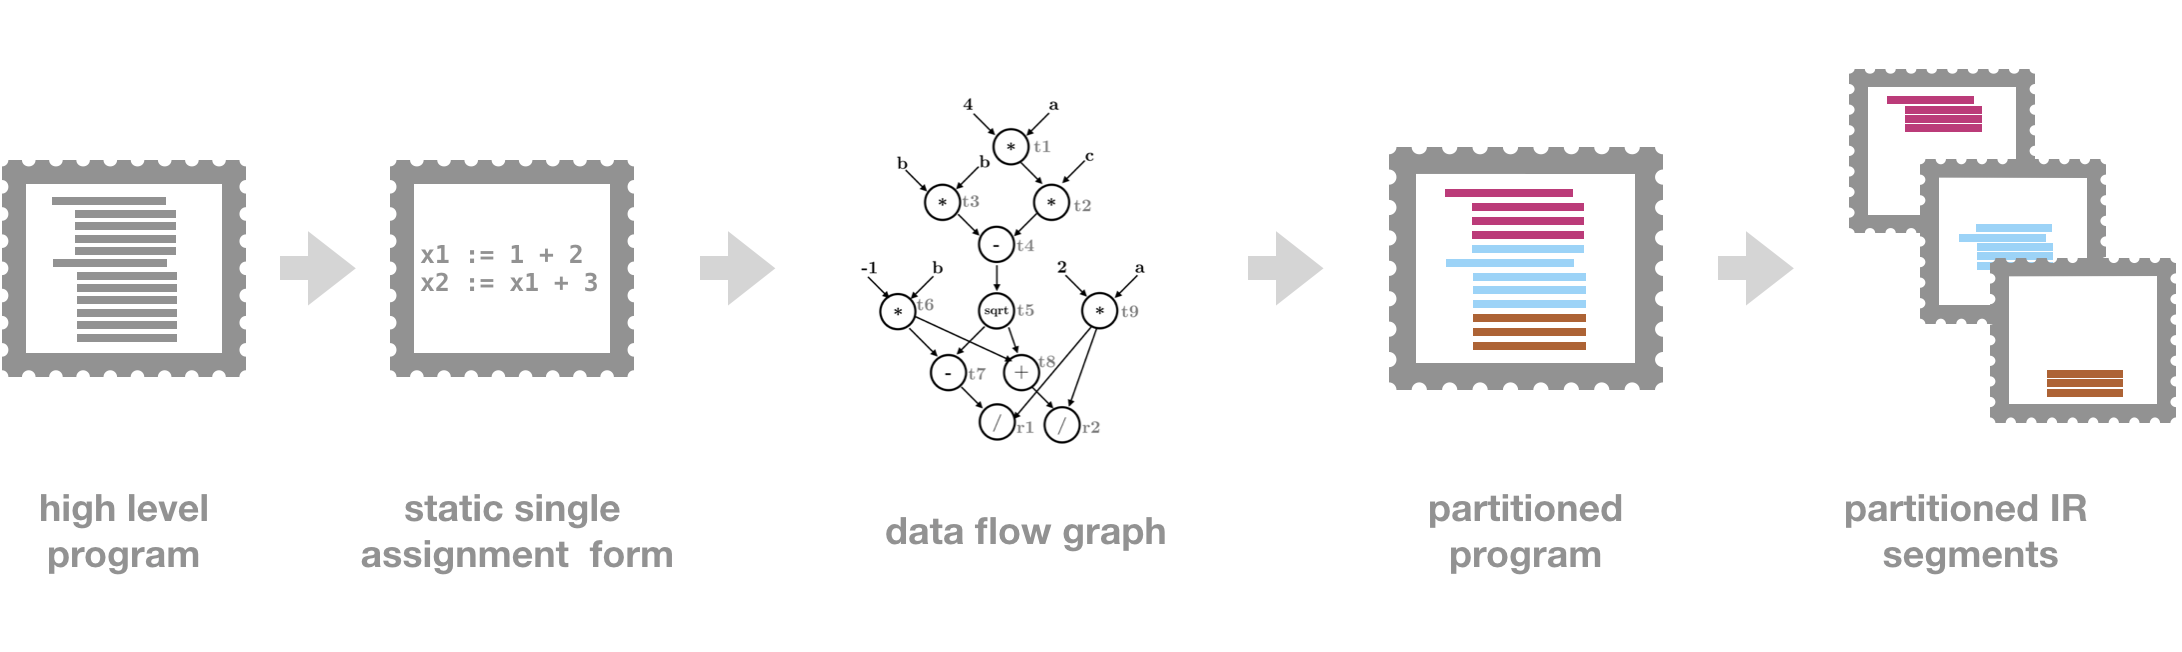
\includegraphics[width=6.5in]{architecture-diagram.png}
\caption{Overall system design for the SSA-Spatial compiler. This paper focused on the transformations between the central three representations: the SSA form, the data flow graph, and the partitioned program.}
\label{fig:design}
\end{figure*}

\subsection{Compilers for Parallelization}
There has been significant work on the general problem of compiling domain-specific, higher-level applications to optimize for particular architectures. For example, for deep learning applications, the TVM compiler can optimize for multiple back-ends, including GPUs and FPGA-based accelerators~\cite{tvm}. However, TVM does not yet support manycore architectures, and it is targeted for machine-learning-specific languages. Halide is a language and compiler designed for image processing that uses stochastic search to schedule computation across CPUs and CPUs~\cite{halide}. In general, parallelization of higher-level applications has focused on commodity hardware including CPUs, GPUs, and increasingly FPGAs, but has not addressed the potential of compiling to specialized, reconfigurable manycore architectures. 
{\note Add citations for TensorFlow and HLS?}

\subsection{Compilers for Manycore Architectures}
Most of the existing compilers for manycore architectures are based on heuristics, rather than program synthesis or constraint solving as a general approach. For example, the RAW compiler (RAWCC) compiles general-purpose sequential programs in C or Fortran to a distributed spacial architecture~\cite{raw}. Because the problem of optimally scheduling computation in space and time is typically NP-complete, RAWCC uses a set of greedy heuristics to create approximate solutions. In particular, they decompose the compilation problem into traditional compiler optimizations, then cluster instructions and merge instruction clusters until they fit within the number of compute units, finally globally partitioning data. However, RAWCC only targets a specific Raw architecture, so each optimization came at the cost of being specifically designed by a compiler engineer. 
{\note Cite TRIPS/Edge from UTAustin}

{\note Consider a section on HLS. Combine with "multi-processor designs from the 1990’s such as CM5, Alewife, Barrelfish"?}

\subsection{Constraint-Guided Compilation}
As described by Lopes and Regehr in \emph{Future Directions for Optimizing Compilers}~\cite{future}, there is increasingly interest in using satisfiability modulo theories (SMT, the core technology behind many forms of program synthesis) and other constraint-based solvers to improve compiler speed, correctness, and generated code quality. However, this area of work is still in the early stages. In particular, because SMT solvers and systems for program synthesis must exhaustively enumerate search spaces, their clients must contend with issues of scalability as problem sizes approach realistic system sizes. 

Alive is a domain-specific language (DSL) for writing efficient and correct compiler optimizations for LLVM, a popular language-agnostic compiler toolchain~\cite{alive}. Alive uses an SMT solver to automatically prove an optimization correct (or, conversely, to provide a counterexample demonstrating its incorrectness). Alive was effective in finding eight previously unknown bugs in an existing LLVM optimization. Optgen is another SMT-based compiler tool that was used to find previously unknown optimizations for GCC, LLVM, and ICC~\cite{optgen}. Souper is a similar, but still preliminary, super-optimizing compiler that uses SMT-solving and also integrates with LLVM~\cite{souper}. Each of these systems focus on optimizing components of existing compilers that mostly target commodity CPUs, rather than leveraging an SMT solver for spatial partitioning for more specialized architectures.

There has also been some previous work using Integer Linear Programming (ILP) constraint solvers to schedule computation across spatial architectures~\cite{ilp}. However, much of the previous focus in that area has been on mapping data flow graphs onto fixed, specific spatial architectures. They are not as flexible, and do not consider architectures that may support reconfiguration. For example, we imagine supporting a manycore architecture where some adjacent cores may pool resources for particularly large pieces of computation. 

Chlorophyll is a synthesis-aided compiler from a custom C-like domain-specific language (DSL) to a particular super-low-power manycore architecture, the GreenArrays GA114~\cite{chlorophyll}. Chlorophyll addresses scalability challenges by dividing the compilation into smaller sub-problems: (1) partitioning computation across cores, (2) layout of logical computation partitions onto physical cores, (3) code separation to divide source code and insert communication code, and (4) code generation to ``super-optimize'' instructions. We plan to leverage the insight from Chlorophyll to separate compiler concerns into phases to enable tractable synthesis that can reasonably scale. However, unlike Chlorophyll, our system aims to support re-configurable architecture rather than than only one specific manycore architecture like the GreenArrays GA114. In separating compilation between logical cores and layout, the Chlorophyll system also loses the opportunity to synthesis some spatial operations. Our compiler combines these two steps, and uses different strategies to handle scaling between them. In addition, the Chlorophyll DSL imposes restrictions particular to the GA114's cores' limitations, including disallowing recursion and arbitrary array indexing. Because the cores in the architectures we imagine targeting will not be as restricted, we would like to be able to support a more flexible high-level programming model (although as described, certainly not within the scope of this semester). 

% \begin{figure}
%     \centering
%     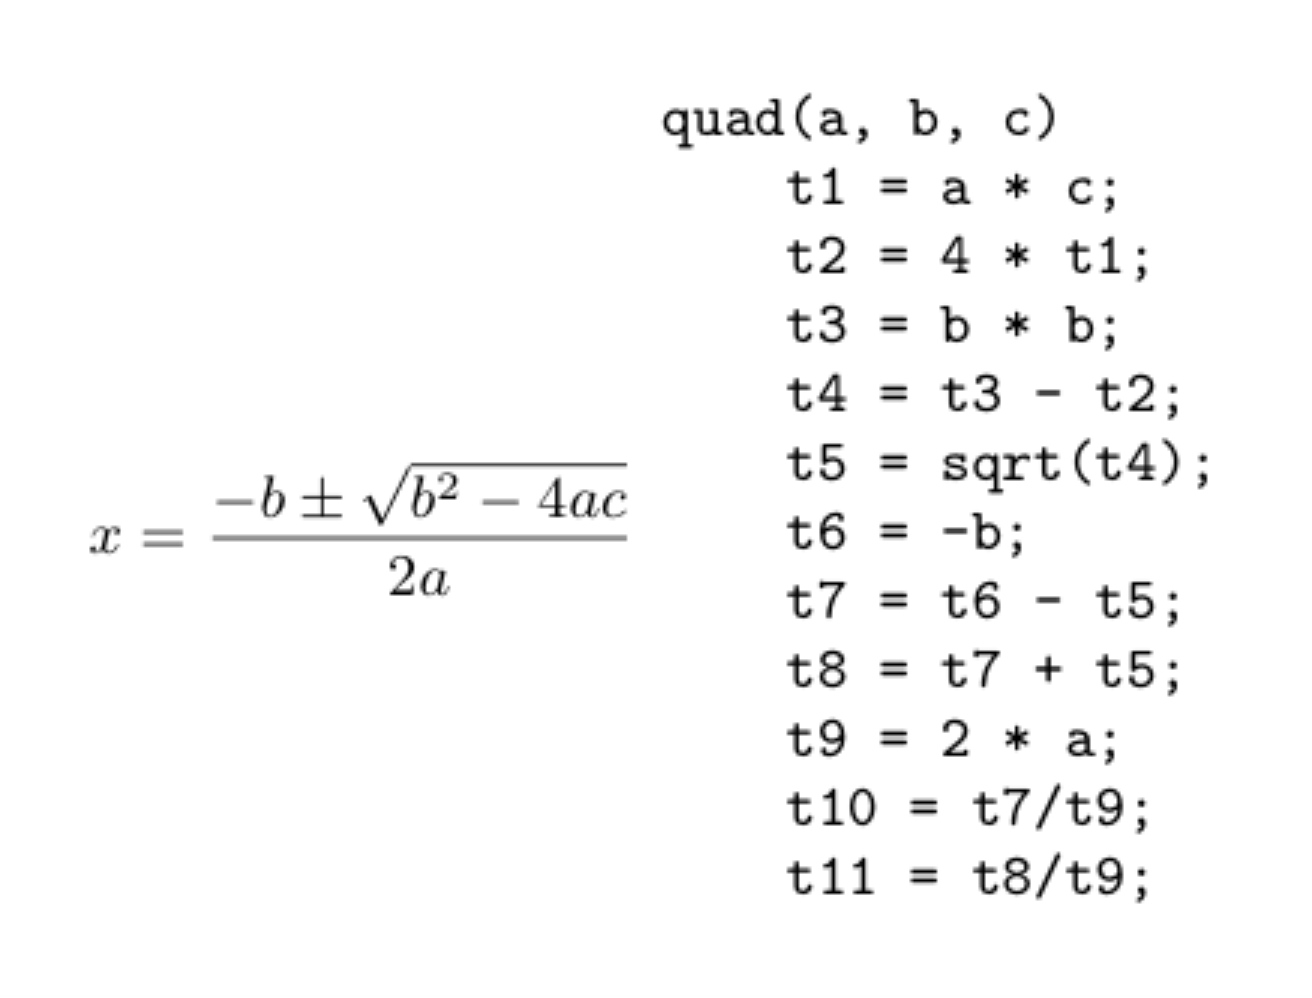
\includegraphics[width=3in]{quadratic.png}
%     $$x=\frac{-b\pm\sqrt{b^2-4ac}}{2a}$$
%     \caption{The quadratic formula (left) expressed as a computation in Static Single-Assignment (SSA) form (right). The roots of the quadratic equation specified by variables $a$, $b$, and $c$ are computed to be the final variables of $t10$ and $t11$.}
% \end{figure}

\section{Design}
One key insight from previous work in using program synthesis for compilation is that in order to scale, compiling must be broken up into several sub-problems. Our system design includes components for (1) compiling from a higher-level language to Static Single-Assignment (SSA) intermediate form, (2) compiling the SSA form into a Data Flow Graph (DFG), (3) mapping that data flow graph over the manycore architecture model using an SMT solver, and (4) generating RISC-V instructions per processor core. This paper focuses on implementing components (2) and (3), and sets the groundwork for completing the end-to-end system in the future. Figure ~\ref{fig:design} outlines this overall system design. 

\subsection{Compiling the Higher-Level Language}
While we would like to eventually support an expressive and flexible high-level language at a similar abstraction level (if significantly less mature) than something like Python, this is not feasible within the scope of a single semester (as specified by the project proposal). Rather, for this paper we focus our analysis and partitioning on a small, simple imperative language that can be built upon incrementally. The initial language only supports a single data types, float, which is used to model integers, floats, and booleans. The language supports branches in control flow via `if`, but does not yet support loops. 

We have created a lexer, parser, interpreter, and compiler for this language using OCaml, a popular functional programming language that offers convenient libraries for language building. We have chosen to leave the extension of this language for later in the course of this project because it is almost entirely language design, and less directly relevant to building efficient systems. 

\begin{figure}[t]
    \centering
    \label{fig:quad}
    \begin{subfigure}[c]{0.49\linewidth}
    \centering
      $$x=\frac{-b\pm\sqrt{b^2-4ac}}{2a}$$
    \end{subfigure}
    \begin{subfigure}[c]{0.49\linewidth}
    \centering
      \begin{verbatim}
quad(a, b, c)
    t1 := 4 * a;
    t2 := t1 * c;
    t3 := b * b;
    t4 := t3 - t2;
    t5 := sqrt t4;
    t6 := neg b;
    t7 := t6 - t5;
    t8 := t6 + t5;
    t9 := 2 * a;
    r1 := t7 / t9;
    r2 := t8 / t9;
    \end{verbatim}
    \end{subfigure}
    \caption{The quadratic formula (left) expressed as a computation in Static Single-Assignment (SSA) form (right). The roots of the quadratic equation specified by variables $a$, $b$, and $c$ are computed to be the final variables of $r1$ and $r2$.}
\end{figure}

\subsection{Static Single-Assignment Form}
Static-Single Assignment (SSA) form is an imperative programming model that requires that every variable is assigned to exactly once, and that every variable is defined before it can be used. This is an especially useful representation for a compiler, because SSA form has a direct translation into a Data Flow Graph (DFG) that models dependencies between operations that process data. Data flow graphs are used in many traditional compiler optimizations, such as reaching definition analysis, where writes to variables that are overwritten before the variable is read can be safely removed from the computation. Figure ~\ref{fig:quad} illustrates a static single-assignment form expression and a data flow graph for the quadratic formula (the equation for finding the roots of a quadratic expression). As you can see, the data flow graph makes data dependencies between different operations explicit. 

\begin{figure}
\centering
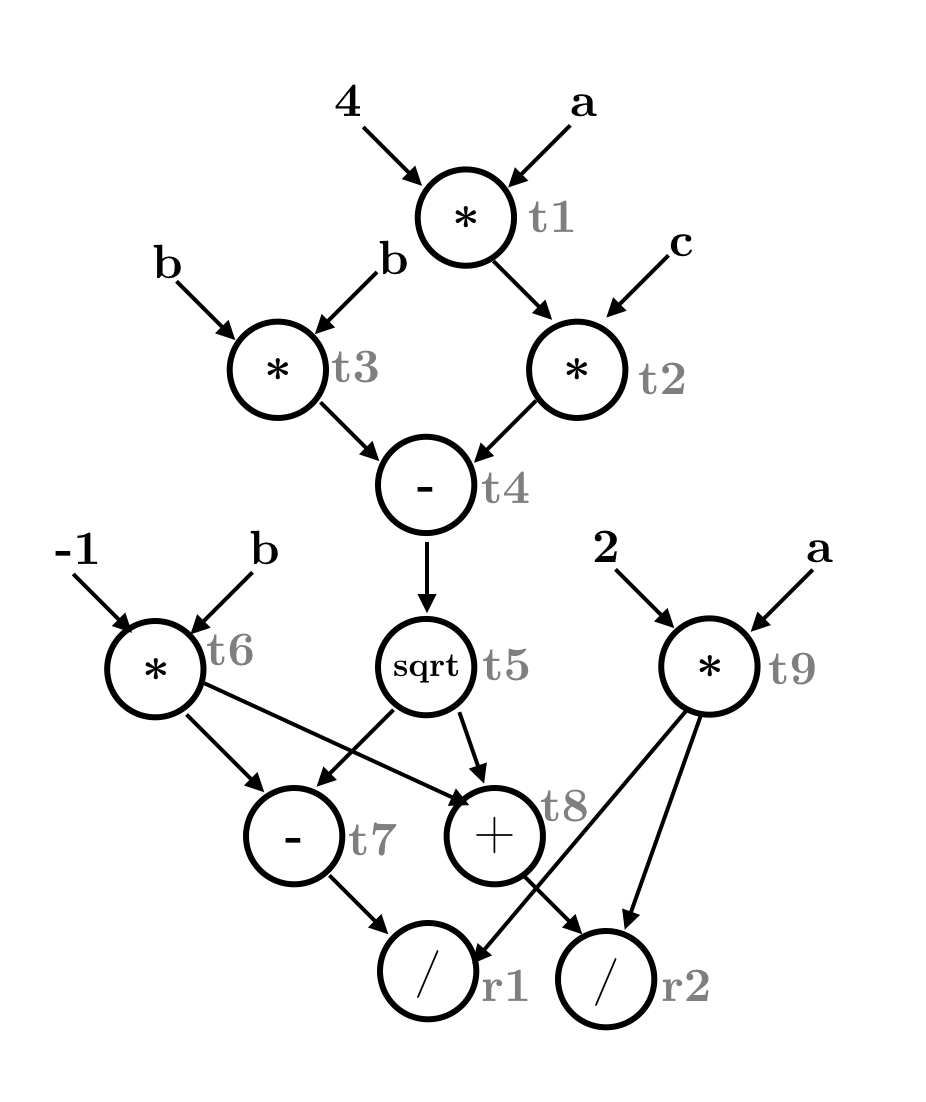
\includegraphics[width=2.7in]{data-flow.png}
\caption{The data flow graph for the quadratic formula computation shown in Figure 2. Each node is labeled with the variable used in the SSA form expression, as well as the operation used.}
\end{figure}

Our first compiler pass transforms the program into a data flow graph representation in order to analyze how to partition computation across cores such that data dependencies are met. In the quadratic formula example, it would be possible for the multiplication operation at \texttt{t1} and the multiplication operation at \texttt{t3} to occur simultaneously on different cores, since they do not have any data dependencies. However, the subtraction operation at \texttt{t4} cannot be mapped to occur simultaneously with the previous operations since it is dependent on their output. This compiler pass is completed via a traditional, syntax-driven program transformation. 

\subsection{Mapping to Manycore}
Once the program representation is in a data flow graph, mapping it to the manycore architecture involves solving a series of constraints on space, time, and communication costs. For constraint solving, we use Microsoft Research's Z3 SMT solver \cite{z3}.

First, we generate a series of constraints that represent the manycore architecture using the SMT Theory of Linear Arithmetic, which models inequalities between integers, and the Theory of Uninterpreted Functions, which models first-order predicate logic. We then Z3 to quantify over all programs that could be generated from the core configuration that satisfy the modeled constraints and are semantically equivalent to the data flow graph. 

Each potential program is modeled such that satisfying instances include an estimated cost for that program partitioning. Once we have a candidate program, we incrementally ask Z3 to find another satisfying instance with the additional constraint that the newer program has a \emph{lower} cost than the most efficient program we have found thus far. We will then repeat this process until no satisfying instances are found. Z3 is able to save internal states between search executions via \texttt{push} and \texttt{pop} commands, which we employ in this strategy of incrementally increasing the difficulty of the cost constraint. We consider a program partitioning \emph{optimal} when Z3 returns that finding a total cost less than the goal is unsatisfiable. However, because we start our synthesis search process with the sequential time cost as the goal, even non-optimal partitionings (where Z3 timesout before reaching a unsatisfiable end goal) represent a speedup over the sequential program.

The strategy outlined above scales to a reasonably-sized manycore grid for small programs. However, the time to compile becomes increasingly prohibitive as the program size grows. As described in our evaluation, our longest microbenchmark of 152 lines of code does not find an optimal solution within 10 hours. In future work, we intend to explore sub-dividing the problem further. For example, we may use a distinct set of constraints to model diving the computation per-core, and then a new set of constraints for communicating across cores. Alternatively, we would like to explore exploiting the symmetry in the spatial layout to accelerate constraint solving. In particular, because the rectangular core grids have rotational symmetry, we hope to eliminate components of the search space that are equivalent to core permutations the solver has already examined.

\subsection{Generating Instructions}
Finally, once we have a program that efficiently maps the data flow graph onto the model of the spatial manycore grid, we need to partition the program into per-core sub-programs in a low-level language. 

We have chosen to base our target low-level language on RISC-V because it is an open and extensible instruction set architecture. The RISC-V distribution also includes a cycle-level simulator, which is described in more detail in the future work section. 

In particular, RISC-V includes a small base of core instructions and numerous optional extensions. New functionality can be added via custom extensions. We plan to base our target language on the RISC-V base plus a small extension to model communication between cores. The compiler pass from the data flow graph and core model to this instruction set will again be heuristic-based program transformation. This transformation will include both mapping the components of the data flow graph into instructions, and adding communication instructions as needed to translate information between cores. We have completed the former component as both a textual output mapping operations to cores, and as a visualization of the data flow graph displaying the partitioned location of each node. The latter component of actually emitting complete RISC-V instructions will be handled in future work. 

\section{Implementation}
We have created a lexer, parser, and interpreter, and compiler for a simple language already consistent with Static Single-Assignment (SSA) form in OCaml.

\subsection{Language Features}
In this language, the only supported type is 64-bit floating-point numbers. Boolean computations are represented with floats, as they are implicitly in many C-based languages. The language supports branches in control flow with \texttt{if} operations, but does not yet support loops or explicit function calls.

One challenge of using SSA form is handling branches with the restriction that every variable is used once, since often the goal of branching is to assign to a single variable in one of two different ways. Our system handles this via the \texttt{phi} operations canonically used in compiler transformations. A \texttt{phi} operation (named to be evocative of \texttt{if}, backward) is used after a branch to select between two variables, based on which control flow path was taken. 

For example, consider the following code in a higher-level language:
\begin{verbatim}
    x := 1;
    if (y) {
        x := 2;
    }
    print x;
\end{verbatim}

Simply replacing each \texttt{x} with a distinctly named variable \texttt{xi} fails to capture that the final print statement should depend on the value set either before or within the branch. This example is represented in our SSA language as:
\begin{verbatim}
    x1 := 1;
    if (y) {
        x2 := 2;
    }
    print phi(x1, x2);
\end{verbatim}

Our interpreter then chooses the left or right hand value for the \texttt{phi} node based on which branch of the control flow was taken during execution time. 

\begin{table}
\begin{center}
  \label{tab:cost}
  \begin{tabular}{cc}
    \hline
    Operation&Estimated Cost (Cycles) \\
    \hline
    \hline
    \texttt{phi}, \texttt{print} & 0 \\
    $\&\&$, $||$, =, !=, <, <=, >, >= & 1 \\
    $+$, $-$ & 2\\
    \texttt{not}, \texttt{negate} & 3\\
    $\times$& 5\\
    \texttt{divide}, \texttt{sqrt} & 10\\
  \hline
\end{tabular}
\end{center}
\caption{Estimated cost per operation}
\end{table}

\subsection{Cost Estimation}
In order to compile the most efficient programs, we need to estimate the cost of both individual operations and communication of data between operations. To do this, we use a series of estimates based on an idealized cycle count. Each unary and binary operation in the language has an associated estimate shown in Table 1. To estimate the cost of communicating pairwise between cores, we use the Manhattan distance between the locations of each core. That is, the total communication cost is the sum of the vertical and horizontal distance between the cores in the spatial layout. 

{\note move insight to results}

One insight we discovered in cost estimation is that the highest costs in the model applicable to specific program have an oversized effect on the efficiency of the program synthesis. Because we begin our search for optimal programs at the upper bound of the sequential program time and (in the best case) end our search when we have found an optimal partitioning, the synthesis engine may have to search for every intermediate cost goal. Reducing our cost estimates (even if we keep the relative costs in between different operations the same) leads to more efficient synthesis, since there are fewer intermediate states in which the synthesis engine must search. 

\subsection{Constraint Generation}

{\note move high-level constraint descriptions in this section to Design}

We construct Satisfiability Modulo Theory (SMT) constraints using the OCaml-Z3 binding library. Currently, the model makes many simplifying assumptions about the manycore architecture. For example, the current constraints allow for each core to read program input from any location, and do not impose restrictions on the memory usage per core. 

We base our constraints on a set of assignments per operation in the data flow graph. Each node $i$ is mapped to a partition, modeled as a symbolic integer $p_i$, and a time interval of symbolic integers $(t1_i, t2_i)$. We first enforce basic physical constraints; for example, that each time integer must be positive. We capture the cost per operation by enforcing that the ending time of an operation $i$, $t2_i$ must be greater than or equal to the starting time $t1_i$ plus the \texttt{operation\_cost} as defined in Table 1:
$$t2_i = t1_i + \texttt{operation\_cost}(i)$$
We model mutual exclusivity between operations per core as logical formulas that each disjoint pair of nodes $i$ and $j$ as:
$$(p_i \neq p_j) \implies (t2_i < t1_j) \vee (t1_i > t2_j)$$
We then add a constraint that for each edge in the data flow graph, the receiving operation must be scheduled after the originating operation \emph{plus} the communication time between their respective core assignments. The standard format for SMT, SMTLib, does not support the mathematical primitives (modulo arithmetic, absolute value) to specify the Manhattan distance directly. While we were able to construct the necessary function from the provided primitives, we found this to be a bottleneck in the synthesis process. Instead, we moved to SMT's Theory of Uninterpreted Functions to specify \texttt{manhattan\_distance} as a function only defined for the integers possibly quantified over in a given synthesis problem---0 to the total number of cores. We can then capture this communication constraint for each edge from operations $i$ to $j$ as:
$$t1_j \geq t2_i + \texttt{manhattan\_distance}(p_i, p_j)$$
Note that this inequality over edges allows for the two inputs for a binary operation to arrive to the operation at different times, as long as they arrive before the computation begins. This assumption may or may not be valid based on the blocking semantics of the hardware. In future work, this is another area we will attempt to make configurable.

Finally, we capture the notion of the total cost of the partitioned program to compare it to our goal. We define a symbolic variable \texttt{latest\_time} to be greater than every ending time $t2_i$. In the future, we may introduce additional factors in the cost model that need to be met for a solution to be considered viable. 

\subsection{Constraint Solving}
We first attempted constraint solving via the SMT \texttt{minimize} command over the \texttt{latest\_time} symbolic integer. However, we found this to be prohibitive in the time for synthesis for larger problems, since it necessitates that the solver find the definitively optimal time. Instead, our compiler now takes an iterative approach.

{\note add an experiment showing the perf comparison here?}

To determine the upper bound of the synthesis search problem, we first compute the estimated sequential time based on the costs in Table 1 (and no communication time, since all computation occurs on one core). We begin by asking the SMT solver for a solution less than the upper bound. Then, based on the resulting latest time of each model, we ask for a solution less than the last know latest time, using the solver's \texttt{push} and \texttt{pop} functionality to save intermediate state. We allow the programmer to set a timeout that applies to each iterative call to the SMT solver. If each iterative solution is found within the timeout, the partitioning concludes when the SMT solver finds the last end goal to be unsatisfiable. In this case, the partition is provably optimal modulo our model's set of assumptions. If any single call to the solver times out, than the last known partitioning is provided as the non-optimal solution. Because we begin the search at the sequential upper bound, this partitioning is guaranteed to be at least as fast as the sequential program running on a single core. 

In practice, this allows the solver to quickly find feasible but non-optimal solutions, then find increasingly narrow gains in each subsequent better solution. We considered instead using binary search to find an ideal solution, but did not find any evidence that the decreased number of goals to consider outweighed the decreased similarity between the saved intermediate states.

\subsection{Visualization}

{\note Probably should remove this whole section.}

\begin{figure}
\centering
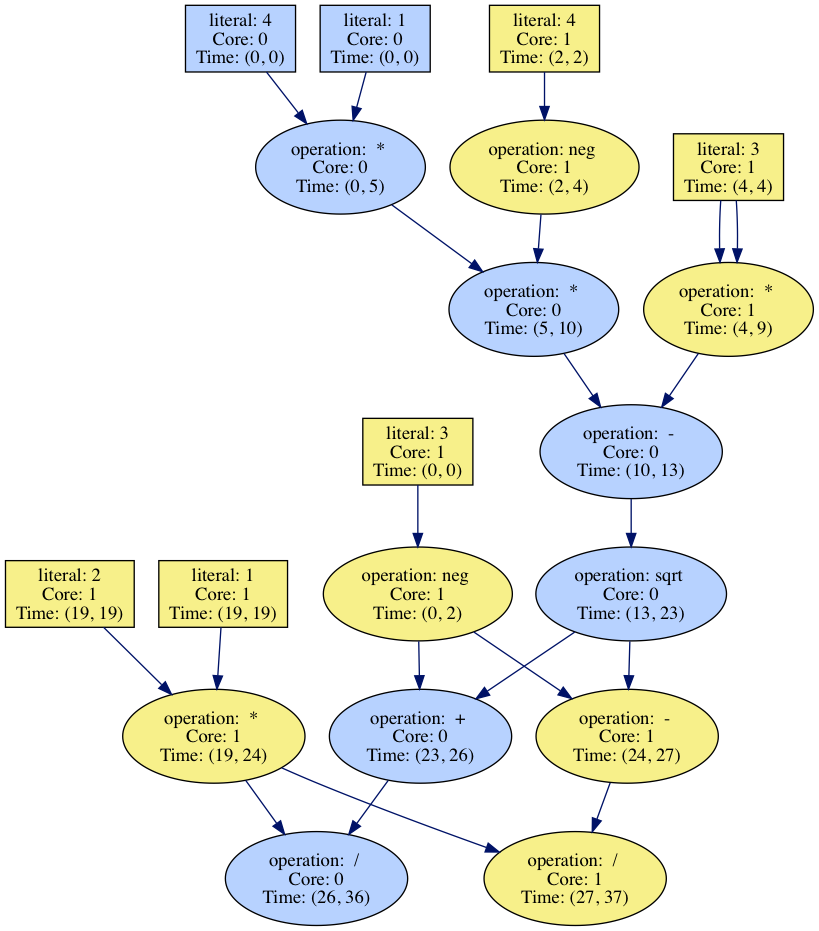
\includegraphics[width=3in]{quadratic-2x2.png}
\caption{An example partitioned data flow diagram visualization that was dynamically generated by the SSA-Spatial compiler. This demonstrates the same quadratic equation example, with $a = 1$, $b = 2$, and $c = -4$. Literal values are shown as square boxes, and operations are shown as ellipses.}
\label{fig:dfg-viz}
\end{figure}

The SSA-Spatial uses OCamlGraph to dynamically create data flow diagrams that display the final partitioning. Each node in the data flow graph is labeled with its operation, the core on which it should run, and the estimated time range during which it will be run. We color-code such visualizations to highlight how pieces of computation are mapped across cores. For example, in Figure ~\ref{fig:dfg-viz}, we can see that one of the longest continuous paths of data-dependencies is mapped entirely to one core, in blue. The remaining computation happens piece-wise on the second core, in yellow, and is forwarded to the primary core.

\section{Evaluation}
We evaluate the performance of the SSA-Spatial compiler across several benchmarks. Because our current source language is limited, we have written custom benchmarks for this paper. However, we have attempted to choose benchmarks that model reasonably distinct workloads. While each microbenchmark under 200 lines of code, synthesizing even short program segments can improve performance. In future work, we can use analysis in the context of a larger compiler to determine bottlenecks in programs that we can isolate to be accelerated using the strategies outlined in this paper.

{\note this evaluation is pretty lame, I need more detail on the microbenchmarks and more info-heavy charts. }

\subsection{Performance Without Timeouts}
Figure \ref{fig:eval-quad-trice} demonstrates the idealized cycle count for a small microbenchmark (repeated applications of the quadratic formula, 50 lines of code). For this experiment, each partitioning completed without a timeout within less than a half hour each. These programs thus represent optimal partitionings (modulo our model's assumptions). We thus estimate that compiling this program for a manycore processor with at least 6 cores (for example, in a 2 x 3 configuration), would result in a 5.0X speedup over the single core performance. For this particular program, providing any additional cores does not further accelerate the idealized time. We determined this both experimentally, and by reasoning about the time of the longest dependency paths within the program's data flow graph. In the future, we would like to augment our synthesis to optionally output the grid size for which additional cores do not offer additional benefit.

\subsection{Performance With Timeouts}
Our longest benchmark, representing a 4x4 matrix multiplication explicitly programmed in our limited SSA form, cannot currently be compiled to an optimal solution without timing out (it did not reach an unsatisfiable end goal within 10 hours). After 10 hours, it found a partitioning with an estimated cost of 141 cycles compared to the sequential upper bound of 464 cycles, representing a 3.3X speedup. We estimate that the optimal partitioning for this benchmark is around 90 cycles. While 10 hours may be a prohibitive compile time for some developer applications, timeout allow the developer to balance their desired speedup with the compile time. Even with a comparatively short timeout of 60 minutes, we are able to gain a speedup from a partitioning of 270 cycles, representing a 1.7X speedup. 
\begin{figure}
\centering
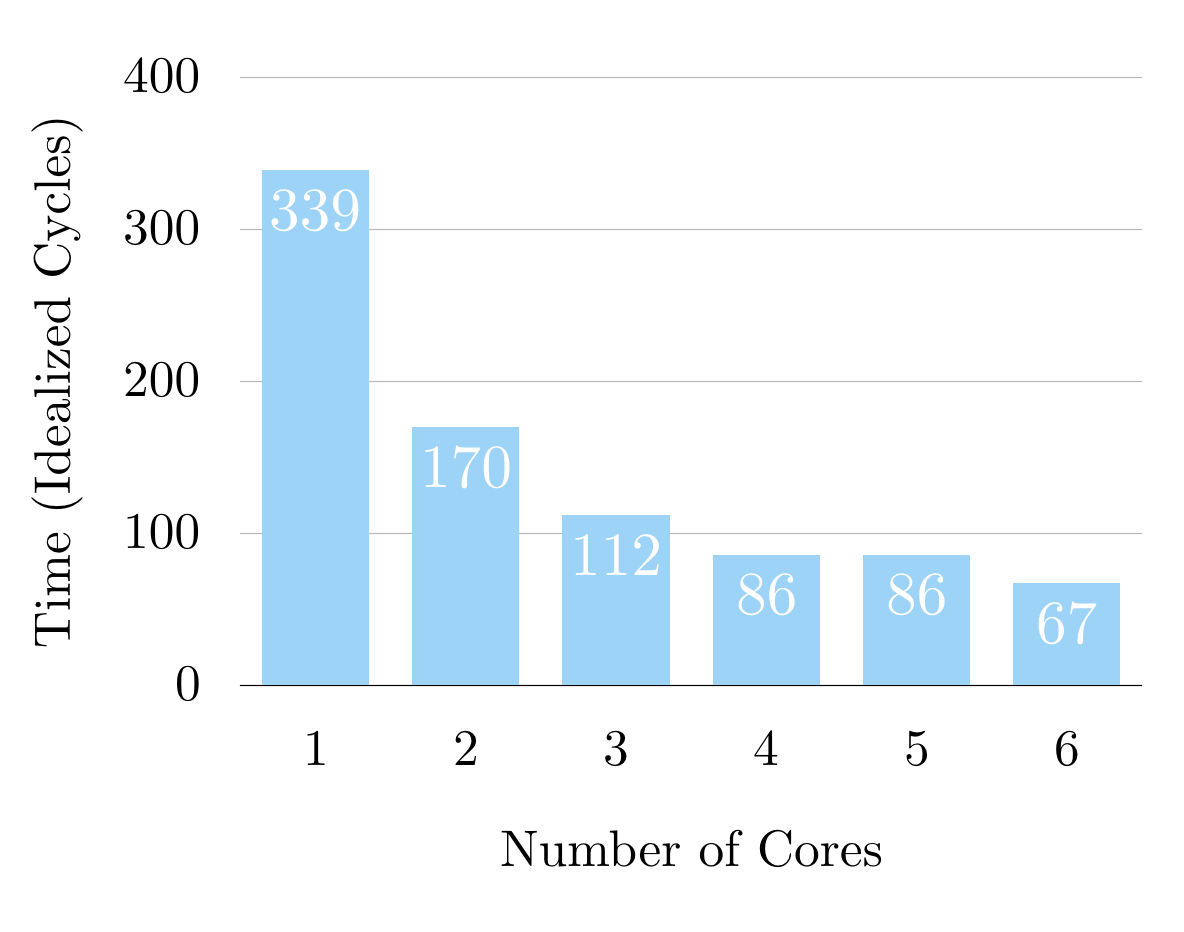
\includegraphics[width=3in]{eval1.png}
\caption{The idealized cycle count for a 50 lines of code program (repeated quadratic formula calculations) compiled across 6 different core configurations, synthesized without a timeout.}
\label{fig:eval-quad-trice}
\end{figure}

\section{Future work}
In the future, we would like to further evaluate the performance of partitioned programs using more detailed simulators. Cornell's Computer Architecture and Programming Abstractions (CAPRA) group is in the process of developing a first-order, cycle-level simulator of the re-configurable manycore architecture. This simulator current supports running arbitrary functions in C++ on each simulator core, as well as communication between the cores. The simulator also allows you to specify per function the estimated cost of that computation. Once the SSA-Spatial compiler generates RISC-V instructions per core, we can run experiments of the execution on this simulator. To do so, we will need to write an interpreter in C++ for the extended RISC-V instruction set. Our existing interpreter for the SSA (static single-assignment) language should be able to inform the implementation of the C++ interpreter. In addition, we will re-use our estimates for the cycle cost per instruction, such that the interpreter can estimate the total cost as well as evaluating the computation.

For comparison, we can then evaluate semantically equivalent computations in the pure RISC-V instruction set by running them on Spike, an open-source RISC-V Instruction Set Architecture (ISA) simulator \cite{risc-v}. We can use the number of cycles output between the two simulators as a proxy for the performance of the compiled code. In addition, Spike allows you to configure the number of simulated cores. Thus, we can evaluate how the performance improvements gained from compiling for a manycore architecture compares relative to gains from adding additional cores within the context of a more traditional operating system and architecture. Finally, with additional benchmarks, we can evaluate how the performance of programs from the synthesis-aided compiler compares to that of equivalent programs: (1) hand-crafted with lower-level languages targeting the manycore hardware, and (2) from more traditional heuristic-based compiler algorithms that target spatial architectures, such as those used by Raw~\cite{raw}. This strategy of comparing results across two distinct simulators is still not an extremely accurate evaluation. In particular, the simulators may make different, influential assumptions about hardware behavior and the associated cycle-level statistics. However, such a simulator comparison is necessary because the targeted manycore architecture does not physically exist yet. In addition, comparing results across simulations will allow us to continue exploring the design space in richer detail. 

In addition, we would ultimately like to allow components of the spatial architecture layout to be symbolic; that is, also leverage program synthesis to inform decisions about how the hardware can be optimally (re-)configured. This involves reworking some components of the Z3 model, such as the number of rows and columns themselves, to be symbolic variables that can be modified later in the analysis. As described previously, we also intend to provider a richer high-level language that can be compiled to the existing SSA form intermediate representation.

\section{Conclusion}
We present SSA-Spatial, a synthesis-aided compiler that partitions programs across a spatial architecture of cores. Our compiler is based on a simple Static-Single Assignment (SSA) intermediate form that can be extended in the future to handle more complex computation. We first transform programs in SSA form to a data flow graph, then produce constraints based on a model of costs for both the operations and communications across cores, and finally use Z3, a Satisfiabiliy Modulo Theory solver, to iteratively find partitions that minimize the cost function. We evaluate the simulated performance of compiled programs estimated by our cost model across a series of microbenchmarks and core configurations. On several small but distinct microbenchmarks, we show speedups of 3.3-5.0X compared to our estimated single threaded performance. In addition, we find that even our longest microbenchmark (152 lines of code) can benefit from a speedup of 1.7X compared to a single core after 62 minutes of iterative compilation. We intend to extend this work in the near future to fully realize the goal of compiling higher-level code to perform efficiently on manycore spatial architectures. 

\section{Acknowledgements} 
Thanks to Professor Adrian Sampson for being a fantastic research supervisor and for many suggestions and reviews of the ideas presented here. Finally, thanks to Professor Hakim Weatherspoon, graduate teaching assistants Danny Adams and Shannon Joyner, and my fellow students for midterm draft reviews of this paper and for a wonderful semester of Advanced Systems. 
\bibliographystyle{abbrv}
\bibliography{refs} 

\end{document}
